\label{ch:desing}
\chapter{Diseño e Implementación}

\section{Limitaciones técnicas para implementar el prototipo}
\label{sec:limitaciones}
Como parte del diseño de la solución, se inicia con una etapa exploratoria. En
esta se anotan manualmente varias aplicaciones de Android, y se identifican
limitaciones del lenguaje Jif para anotar código del framework Android.
Tales limitaciones son adicionales a las características del lenguaje Java no
reconocidas por Jif, a continuación se describen tanto las encontradas, como las
especificadas en el manual de referencia de Jif.

-\textit{Características del lenguaje Java no soportadas por jif}\newline
Si bien, el sistema de anotaciones de Jif hace extensiones al lenguaje java,
permitiendo la evaluación de políticas de confidencialidad e integridad para
aplicativos implementados en dicho lenguaje, el manual de referencia de Jif
precisa las características del lenguaje Java no soportadas\cite{jifRef}. Estas
son:
\begin{itemize}
  \item nested classes: clases que son definidas dentro de otras clases.
  \item initializer blocks: bloques de código declarados dentro de la clase pero
  sin pertenecer a ningún método, dependiendo de si se trata de static
  initialization blocks, su código es el primero en ejecutarse, una vez se
  carga la clase; o si se trata de instance initialization blocks, su código se
  ejecutan cada vez que se crea una instancia de la clase.
\item threads.
\end{itemize} 
Partiendo de estas precisiones, aplicaciones Android que presenten tales
características son excluidas del grupo de aplicaciones a analizar(conjunto de
aplicaciones evaluables) mediante la herramienta propuesta.

% Adicional a las limitaciones de jif frente a características propias del
% lenguaje Java, tras experimentar la anotación manual de una serie de
% aplicaciones Android, se identifican varias limitaciones técnicas para la
% anotación de de las mismas. Entre las limitaciones identificadas están:\newline 

- \textit{Soporte para sobreescritura de métodos}\newline 
En la construcción de aplicaciones Android, según el componente que se esté
implementando(activities, content providers, receivers, services), se requiere
sobreescribir métodos de la clase que extienda el componente. Así, cuando se
define un componente tipo Activity, que debe extender de la clase Activiy.java, 
se sobreescriben métodos como Oncreate. Cada que se sobreescribe
un método se utiliza el statement @Override, con el cual se informa al
compilador de Java que el método es sobreescrito. No obstante, al implementar la
versión Jif de aplicaciones Android con dicho statement, el compilador de Jif
no lo reconoce. La dificultad que se presenta está en el reconocimiento del
statement(carácter @ y clase Override), y no en la sobreescritura de métodos,
puesto que Jif soporta tal característica. El soporte para la sobreescritura de
métodos es confirmado con una sencilla prueba, anotando la clase Activity.java
del framework Android (con un único método, el método Ocreate), e implementando
la versión Jif de una aplicación Android que extiende de tal clase, en la cual
se define una actividad y sobreescribe el método Oncreate.
Cuando se comenta la sentencia @Override, el compilador de Jif identifica la
sobreescritura del método y reporta comentarios para el flujo de información.\newline 
Al investigar el por qué Jif no reconoce tal sentencia, se encuentra que dentro
de las clases Java estándar soportadas por el compilador de Jif, no está
contenida la clase java.lang.Override.\newline
Las clases Java estándar pertenecientes a los paquetes io, lang, math, net y
sql; para las que el compilador Jif brinda soporte, vienen implementadas con
anotaciones en el directorio sig-src, directorio que forma parte de la
distribución del compilador de Jif con que se esté trabajando.\newline
Una alternativa para permitir el análisis de flujo de información entre métodos
que se sobreescriben, es comentar las líneas del programa que contengan la
sentencia @Override, puesto que, al no ser reconocida por el compilador de Jif,
es la generadora de errores de compilación.

- \textit{Casting entre tipos EditText y View}\newline
El framework de Android cuenta con diferentes clases para manejar las interfaces
gráficas que presenta al usuario, entre las cuales se encuentran EditText y
View. View es la clase principal para la creación de widgets, necesarios para la
implementación de componentes interactivos en las interfaces de usuario(UI).
EditText permite adicionar campos de texto editables en UI. El casting entre los
tipos de datos que representan ambas clases, se hace cuando la aplicación debe
procesar datos provenientes de campos en las interfaces del usuario, por ejemplo
como se observa a continuación:
\begin{lstlisting}
EditText editPassword = (EditText)findViewById(R.id.password);
String password = editPassword.getText().toString();
\end{lstlisting}
la interfaz de usuario(que es de tipo View) contiene un campo R.id.password, y
para manipular la información que almacena, debe ser de tipo EditText, siendo
necesario un casting de tipo View a tipo EditText. La dificultad que se presenta
con este tipo de casting es que para el sistema de anotaciones de jif no es
válido. Luego de probar con la anotación manual de ambas clases, tratando de
dar soporte a este tipo de casting, sin obtener resultados satisfactorios, se
opta por ``simular'' estos casos, es decir, si el tipo de dato de una variable
es de tipo EditText, se crea una varible tipo String con un valor determinado,
así se omite el casting y se puede analizar el flujo de información.

- \textit{Clase nested R}\newline
El framework de Android utiliza identificadores para hacer referencia a recursos
utilizados por la aplicación, recursos como strings, widgets y layouts, tales
identificadores son autogenerados en la clase R.java, allí cada recurso es
descrito como una clase individual. Al tratarse de una clase nested, la clase R
no puede ser anotada con jif. Esto puede solucionarse implementando una
versión Jif generalizada de la clase R, que contenga los recursos utilizados en
una aplicación, definidos como variables y no como clases.

- \textit{Sources y Sinks}\newline
En el diseño inicial de la solución se propone utilizar SuSi para clasificar
los sources y sinks en las aplicaciones a analizar, sin embargo, partir del
extenso conjunto de sources y sinks, clasificados por SuSi para la API de
Android, implica una mayor complejidad en el análisis, puesto que, en un
aplicativo todo el código que le conforma puede hacer parte de sources o de
sinks. Adicional a lo complejo que se puede tornar el análisis, los sources y
sinks a considerar deben depender de la política de seguridad a evaluar. En ese
orden de ideas, resulta más viable tomar un subconjunto del listado proveído por
SuSi, partiendo de los sources y sinks que evalué la política de seguridad que
se defina.

- \textit{Enhanced for loop} \newline
Además de soportar la estructura de control for, el lenguaje Java permite el uso
de enhanced for, que es utilizado para simplificar la iteración en arrays y
colecciones, por ejemplo:
% \begin{lstlisting}
% char c[] = imei.toCharArray();
% for (int i = 0; i < c.length; i++) {
% 	obfuscated += c[i] + "_";
% }          
% \end{lstlisting}  
\begin{lstlisting}
for(char c : imei.toCharArray())
obfuscated += c + "_";
\end{lstlisting}
A diferencia de Java, Jif no soporta el enhanced for.\newline
Debido a que ambas sentencias de control son equivalentes, la solución que se
propone para poder analizar flujo de información en los aplicativos Android que
contengan dicha estructura de control, es generar el equivalente del programa
haciendo uso del for, de este modo se cambia la sintaxis sin afectar la lógica
del aplicativo a analizar.

- \textit{Otras limitaciones} \newline
Adicional a las limitaciones descritas anteriormente, para las cuales se propone
una solución, se identifica que Jif no soporta la sintaxis utilizada para
definir estructuras de datos HashMaps, LinkedList y Sets, que en Java se definen
de la siguiente manera:
\begin{lstlisting}
Map<String,String> hashMap = new HashMap<String, String>();
List<String> listData;
Set<String> phoneNumbers = new HashSet<String>();
\end{lstlisting}
Jif tampoco permite la definición de interfaces como argumentos de un método. El
siguiente fragmento de código  en una aplicación Android, muestra la definición
de una interfaz pasada como parámetro al método setOnClickListener.
\begin{lstlisting}
   Button button1= (Button) findViewById(R.id.button1);
   button1.setOnClickListener(new View.OnClickListener() {
   ...
   .....}  });
\end{lstlisting}
En estos casos, la dificultad está en encontrar una sintaxis que permita obtener
la versión equivalente del programa que las contenga. A lo que se suma, la falta
de documentación disponible para solventar los mismos. En consecuencia, se omite
del conjunto de aplicaciones evaluables, aplicaciones Android que requieran en
su implementación las estructuras de datos descritas.\newline

%- \textit{Paso de statements dentro de los argumentos de un método
%(\{\}):}\newline

\section{Diseño de la solución} 
\subsection{Definición de la política de seguridad}
Detectar si una aplicación Android(perteneciente al conjunto evaluable) presenta
flujos de información entre, información con nivel de seguridad alto e
información con nivel de seguridad bajo.\newline
Detectando fugas de información catalogada con nivel de seguridad alto, vía:
canales creados durante el control de flujo del programa(flujos implícitos),
mensajes de texto y mensajes de Log.\newline 

\subsection{Consideraciones para verificar el cumplimiento de la política
mediante Jif} 
\label{subsec:consVerPol}
Teniendo definida la política de seguridad a verificar, se describen
elementos influyentes en el diseño de la solución.

\textit{Versión de la API de Android}\newline
Las aplicaciones utilizadas para los experimentos previos a la implementación
del prototipo, y las aplicaciones a anotar con el mismo, se realiza partiendo de
la versión Android 4.2.2(API Level 17).

\textit{Versión del compilador de Jif}\newline
se parte de la versión 3.4.2 del compilador de jif, para llevar a cabo tanto los
experimentos previos como el análisis de las aplicaciones anotadas por el prototipo.

\textit{Diferencia entre una aplicación Android y una aplicación Java
convencional}\newline 
En esencia, una aplicación Android es una aplicación Java con interfaces
descritas en XML, que para ser ejecutada necesita del framework de Android,
porque este le provee acceso al hardware del dispositivo y funcionalidades del
sistema.\newline 
Por otro lado, Jif permite hacer seguimiento al flujo de información de una
aplicación Java, extendiendo el lenguaje mediante labels de seguridad.\newline
Para analizar flujo de información de una aplicación Android mediante
Jif, es importante mencionar que mientras una aplicación Java convencional
cuenta con un único punto de entrada para iniciar su ejecución, esto es, la
clase principal donde se implementa el método main; una aplicación Android puede
tener más de un punto de entrada, generados a partir de los diferentes tipos de
componentes que le integren(Activity, Service, Content Provider y Broadcast
Receiver). La necesidad de interacción del usuario para activar tales puntos de
entrada varía acorde al tipo de componente, así, en el caso de componentes tipo
Activity su ejecución sólo inicia hasta que el usuario interactúe con la
actividad, y para manejar dicha interacción, la API Android provee el método
OnCreate. De otro modo, componentes tipo Service y Broadcast Receiver, inician
su ejecución a través de los métodos OnStartCommand y OnReceive,
respectivamente, sin necesidad de interacción del usuario.\newline 
{ \color{black} {Teniendo en cuenta lo anterior, se asume que la aplicación a
evaluar tiene un único punto de entrada, que depende del tipo de componente que
implemente.} }

\textit{Chequeo de excepciones tipo Runtime}\newline
En lenguaje Java las excepciones tipo Runtime tales como NullPonterException, no
son verificadas a tiempo de compilación, sin embargo, buscando evitar la
generación de canales encubiertos mediante las mismas, Jif si las verifica. 
En consecuencia, si un programa requiere excepciones NullPointerException,
ClassCastException y/o ArrayIndexOutOfBoundsException, el programador debe
declararlas en el programa, de lo contrario, el compilador de Jif genera error.
Para las aplicaciones a analizar, se espera que el desarrollador haya
especificado las excepciones necesarias.

\textit{Información considerada con nivel de seguridad alto}\newline
Para verificar el cumplimiento de la política de seguridad a evaluar se parte de
un conjunto de sources, caracterizados por dar a conocer información del usuario, 
considerada como privada o sensible. Los métodos que integran el conjunto de sources son: 
getDeviceId, getSimSerialNumber, findViewById, getLatitude, getLongitude y
getSubscriberId. Adicional a estos métodos, se incluye el tipo de dato EditText,
si y sólo si, el campo UI al que referencia corresponde a un campo tipo
textPassword, es decir, un campo que almacena contraseñas.

\textit{Canales que muestran información con nivel de seguridad bajo}\newline
La información enviada a través de mensajes de texto y la información conocida
tanto a través de mensajes de Log, como a través de canales generados por el
control de flujo del programa, tiene en común que debe poder ser conocida por
terceros. En consecuencia, se considera que estos canales deben dar a conocer
información con nivel de seguridad bajo.\newline
En el caso de mensajes de texto y mensajes de Log, se hace referencia
específicamente a las clases Log y SmsManager de la API de Android.

\textit{Evaluación del flujo de información}\newline
Para evaluar el flujo de información, se asume que todos los métodos definidos
en la clase serán invocados, y por tanto, todos son incluidos en el análisis.\newline 
Esta decisión de análisis busca evitar el paso inadvertido de flujos de
información, generados por omisión.

\textit{Acceso a métodos de sobreescritura.}\newline
Los métodos de las clases Activity, Service y BroadcastReceiver, son métodos
que se pueden sobreescribir, todo programa Android que extienda de tales clases
debe poder utilizarlos.


\subsection{Pasos para el diseño de la solución}
\label{subsec:pasosSol}
\begin{figure}[t!]
	\begin{center}
	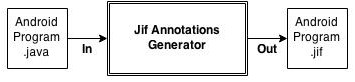
\includegraphics[width=7cm]{desingSolution.jpg}
	\end{center}
	\caption{Entradas y salidas para el generador de anotaciones.}
	\label{fig:desingSolution} 
\end{figure}
Una vez clarificadas las limitaciones técnicas y los elementos a considerar para
el diseño de la solución, se describen los pasos necesarios para la
implementación de la misma. Como se ilustra en la figura
\ref{fig:desingSolution}, la solución a implementar consiste en un anotador de
aplicaciones Android, que recibe como entrada una aplicación
Android(perteneciente al conjunto evaluable), y devuelve la versión Jif del
mismo, el cual contiene las anotaciones para evaluar la política de seguridad
definida.\newline

\textit{Paso uno: hacer que Jif reconozca determinadas clases de la API de
Android}.

\begin{figure}[h!]
	\begin{center}
	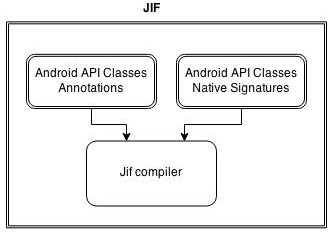
\includegraphics[width=5cm]{desingSol-steps1.jpg}
	\end{center}
	\caption{Tipos de anotación necesarias para implementar la solución.}
	\label{fig:desingSol-steps1}
\end{figure}

\begin{figure}[t!]
	\begin{center}
	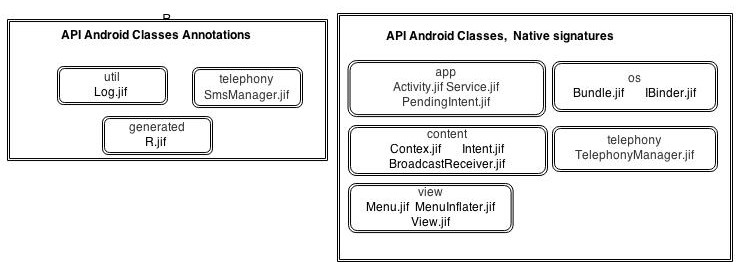
\includegraphics[width=12cm]{desingSol-step1-details.jpg}
	\end{center}
	\caption{Diseño de la solución paso 1. Ilustra las clases especificas de la
	API de Android, anotadas manualmente.}
	\label{fig:desingSol-details}
\end{figure}
Adicional al mecanismo de anotación que se maneja en Jif, en que para hacer
análisis al flujo de información de un programa Java, se debe implementar la
versión del respectivo programa para Jif. También es posible adicionar clases
Java ya existentes, utilizando signaturas nativas para que el compilador Jif las
reconozca, esto es: generando una versión Jif de la clase java, donde se
declaran constructores y cuerpo de los métodos a utilizar de la clase fuente
Java.\newline
Para el presente trabajo se utilizan ambas opciones de anotación. Tal como se
ilustra en la figura \ref{fig:desingSol-steps1}. 
El criterio para decidir que se anota de una u otra forma, depende de lo que
represente la clase Android para verificar la política de seguridad establecida.
Las clases Log y SmsManager, que representan canales para conocer información,
son anotadas de forma no nativa. La opción de anotación nativa se utiliza para
librerías Android, por ejemplo la clase TelephonyManager necesaria para utilizar
el método getDeviceId. En la figura \ref{fig:desingSol-details} se especifican
clases de la API Android a anotar.\newline

\textit{Paso dos: Definir Autoridades y forma de anotación del programa Android
a analizar.}\newline
Una clase Android tendrá una Autoridad máxima(un principal), en este caso Alice,
así que, información con nivel de seguridad alto deberá pertenecer a dicha
autoridad.\newline
Jif hace seguimiento al flujo de información del programa, asociando un label
de seguridad al program counter de cada sentencia y expresión del programa,
program counter(pc) label. Este pc es afectado por el label de seguridad que se
especifique en la declaración de variables y métodos\ref{subsec:JifSintax}. 
Partiendo de que Jif se fundamenta en labels de seguridad para hacer seguimiento
al flujo de información del programa, es necesario definir los labels a
anotar para métodos y variables del programa.\newline
En el caso de variables con nivel de seguridad  alto, la anotación debe
ser:\newline
\emph{ type\{Alice:\} varName; }\newline
Para el resto de variables, entran a jugar las anotaciones definidas por Jif
acorde al contexto donde están definidas.\newline
Ahora en el caso de los métodos, la anotación varía según si el método debe
influenciar(acceder, modificar) o no, información anotada con nivel de seguridad
alto.

En base a lo anterior, se define un algoritmo de anotación que se condensa en un
generador de anotaciones; y se fundamentado en las siguientes
definiciones:\newline \textit{Definición A:} anotación de variables con nivel de
seguridad alto:\newline modifier type\{Alice:\} varName;\newline 
\textit{Definición B:} métodos que se sobreescriben. El sistema de anotaciones
de Jif exige que el nivel de seguridad del método desde donde se invoca la
sobreescritura de un método, no debe ser menos restrictivo que el método a
sobreescribir, y los métodos a sobreescribir deben poder ser invocados desde
todo programa Android, siguiendo con este principio, y buscando que jif no
limite el flujo de información, estos métodos deben ser anotados con BL
público(\{\}).\newline 
\textit{Definición C:} anotación de métodos con sources\newline
Los labels para la definición del método(BL, EL, AL )se anotan de la
siguiente manera:\newline modifier type
nameMethod\textit{\{Alice:\}} type\textit{\{Alice:\}}
( arg1,.....type\textit{\{Alice:\}}argn ) \{\}\newline Si dentro del método se
definen arrays, sus respectivos BL y SL, deben ser anotados así: modifier type\{Alice:\}[ ]\{Alice:\}\newline
\textit{Definición D:} anotación de métodos que no reciben información del
source. 
nameMethod\textit{\{\}}(
type\textit{\{Alice:\}}arg1,.....type\textit{\{Alice:\}}argn ) \{\}\newline
Teniendo claras las anteriores definiciones, los pasos para el algoritmo son los
siguiente:\newline
(1) Identificar sources de la clase. Si se encuentran sources continuar con
los pasos (2) a (4), sino, continuar con paso (2) y aplicar definiciones B y
D.\newline
(2) Identificar el total de métodos de la clase.\newline
(3) Del total de métodos listar los que son invocados con el source.\newline
(4) Del total de métodos listar los que no son invocados con el source.\newline
(5) Aplicar definición C a listado del paso(3).\newline
(6) Aplicar definición D a listado del paso (4).\newline
(7) Aplicar definición B. \newline
(8) Aplicar definición A a listado del paso (1).

\subsection{Descripción implementación prototipo}
-Diagrama de clases o descripción

